\subsection{Rest of the Stuff}

%\section{Malleable TOHTN Planning}
- as mentioned by \cite{sanders2022decentralized}, upgrading a moldable to a malleable job is easy for portfolio solvers where a number of parallel but independent search strategies is involved
- \cite{sanders2022decentralized}, the application itself is responsible to handle the removal/ addition of workers

- upgrade from moldable to malleable task according to \cite{feitelson1997job} as introduced in section \ref{prelim: malleability}
- we can no longer assume that messages always arrive and get a response
- we want to achieve completeness
- when sending a message, we always want to send it to another 
%\subsection{Adapting CrowdHTN to a Malleable Environment}
As discussed in section \ref{prelim: crowdhtn}, CrowdHTN in its original form is a moldable program, with the number of parallel workers fixed for each single execution. To adapt CrowdHTN to work as a malleable program within Mallob, we have to address three key concerns.
\begin{enumerate}
	\item Messages sent to workers who are suspended or terminated before it arrives
	\item Integrating new processes to work efficiently
	\item Dealing with workers dying without loosing completeness
\end{enumerate}
To help understanding, this section explicitly discerns between Mallob workers and Crowd workers. \todo{more terminology}
\paragraph{Messages sent to dead workers}

\subparagraph{Receiving worker stays dead}
\todo{adapt intro to the split into 'stays dead' and 'got replace'}
As Mallob runs each worker in a different processes communicating via message passing, we never have a full view of the current global state of our process, i.e., which other Mallob workers are assigned to the same job. Instead we only ever get information about this that might be outdated. As a result, when a message such as a work request is sent to another worker, we cannot be sure that the receiving worker is in a position to actually respond. Luckily, Mallob does provide us with a mechanism to detect such messages. Each Mallob worker knows which job it currently works on and all messages are tagged with their job as well. If a message belonging to job $J_i$ is received by a worker working on job $J_k, k \neq i$, the message is simply tagged with a \textit{returned to sender} flag and sent back. \\
Now we can simply adapt CrowdHTN to deal with each message both if it is received normally and if it is received as a return message. On normal messages, nothing changes. On return messages we do the following:
\begin{itemize}
	\item \textbf{Work request}: we treat this like a negative response. This means we set the \textit{has active work request} flag to false and simply send out another work request at the next chance.
	\item \textbf{Positive work response}: this is the node we sent out ourselves. As to not loose any information, we simply re-insert the node at the front of our local fringe. While this may slightly change the order of the nodes at the front, we expect the number of outgoing work packages at any point to be small and the disturbance to be limited. In case of random searches, it should not negatively affect our algorithm.
	\item \textbf{Negative work response}: we do not have to care about this and can simply ignore it.
	\item \textbf{Ack}: we do not have to care about this and can simply ignore it.
\end{itemize}
While this mechanism should deal with most cases of workers dying, we can always construct pathological cases in which the return message mechanism fails. One such exchange can be seen in graphic \ref{malleable: lost message}. One way of dealing with this would be to change the way Mallob handles messages whose receiver is no longer valid. E.g., if a return message was delivered to a worker who changed jobs in the meantime, one could instead find out the root worker of the accompanying job and send the message there instead.
\todo{ref that the root always lives at least as long as everything else}
This way no information would be lost until we decide to terminate the whole job at which point this would be unavoidable and okay by the user. To avoid having to change Mallob, we instead elected to make our adaptation of CrowdHTN resistant to such information loss.
\todo{write about loop detection and restarts here}
\begin{figure}
	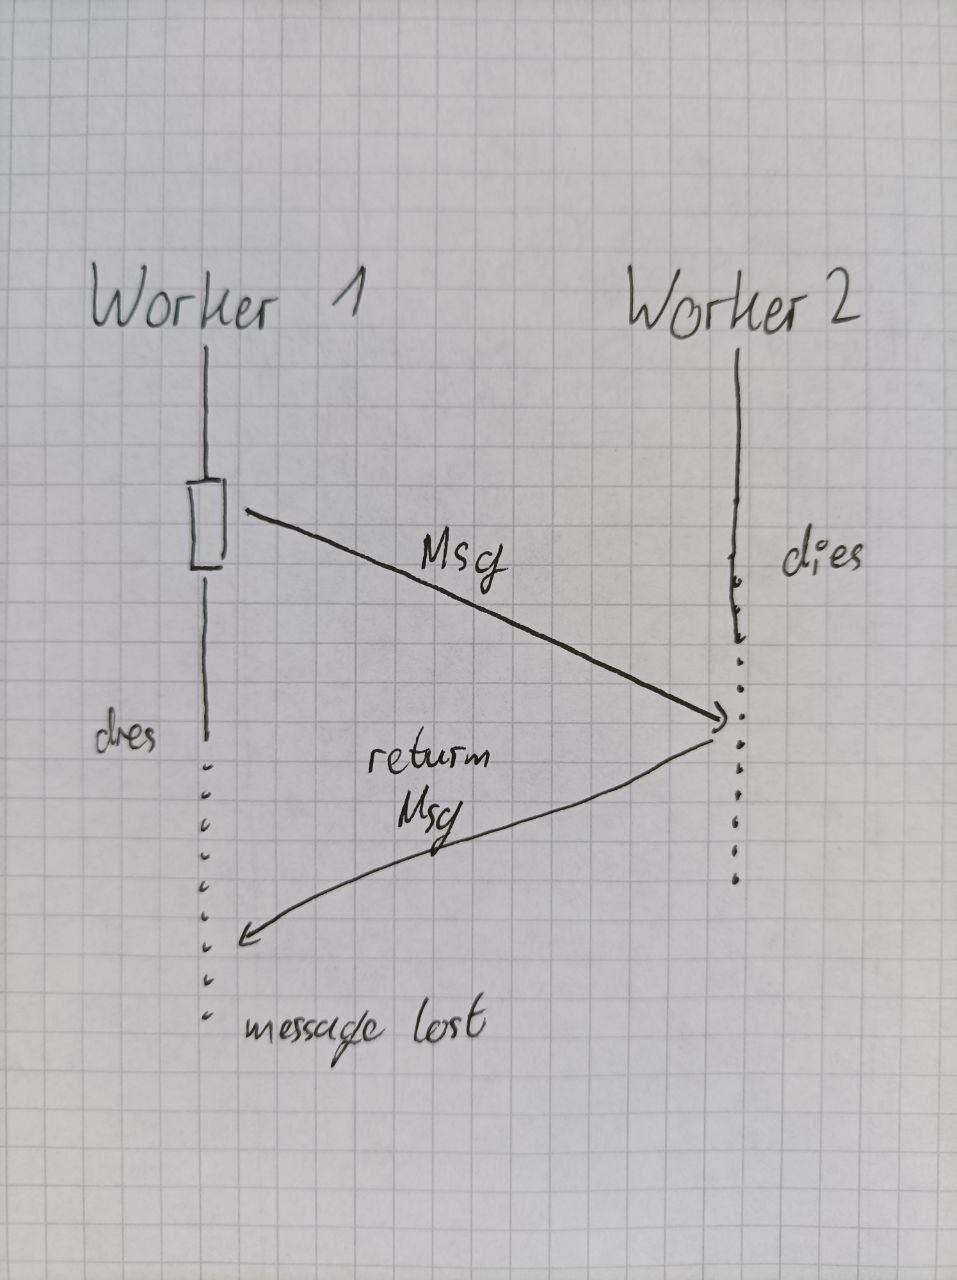
\includegraphics[width=0.6\textwidth]{images/prelim/malleable_lost_message}
	\caption{Example diagram of a lost message}
	\label{malleable: lost message}
\end{figure}

\subparagraph{Receiving worker gets replaced by a new worker}
- we have no way to detect this case
- some messages we can absorb
	- a lone ack: we don't care, instead of decreasing the number of outgoing packages we set the count to max(0, count -1)
	- a work request: can be responded to as if it was meant for us
	- work responses pose a problem: a node may send out a work request, die, a new node starts, starts it's own work request and receives the response afterwards
		- dafuq, this is complicated
		- buuut, it can happen
		- what if we just accept it? Worst case we get two positive responses, take both of them and deal with it
		- number can decrease again if two negative responses arrive before sending off a new request
		- cycle will interrupt anyways upon the first positive response (yay!)
	- everything is fine dot jay pee gee
\todo{are messages received by suspended jobs?}

\paragraph{Integrating new workers}
As CrowdHTN uses work stealing to distribute work and perform load balancing, new workers can be seamlessly integrated into a running job. Upon construction all workers are treated the same, whether they are part of the initial batch or appear at a later point. The root worker is initialized with the initial search node, all other nodes are empty. To get new work, a worker sends a work request to a random other node and then goes from there. The very same process can be used to integrate a new worker.
\paragraph{Dealing with the information loss of dying workers}
\todo{Mallob simply solves the same job on every node, parallelism is trivial, no need to worry about lost information}
As mentioned before, dying workers can lead to a loss of information. A previous paragraph discussed what this means for messages sent between workers. There is a second part of dying workers that we need to adjust to - the loss of the local fringe. There are three main ways in which we could deal with this loss.
\begin{itemize}
	\item Communicate the local fringe to the parent or root worker
	\item Communicate the root search node of the local search to the parent or root worker
	\item Accept the loss of information and thus of parts of our search space
\end{itemize}
We will discuss these strategies one by one.
\subparagraph{Communicate the local fringe}
- cleanest solution in a way
- no information is ever lost
- problems:
	- time needed for encoding the fringe is unbounded
	- an efficient encoding of the shared open tasks and world state would complicate the implementation
	- we need to ensure that the message containing our local fringe is not lost
		- i.e. it has to be sent to the root worker as it is guaranteed to live as long as anyone else
		- this imposes additional memory pressure on our root if many nodes terminate
\subparagraph{Communicate the root back}
- this is guaranteed to not loose any information
- however, we will have to re-do some work
- communication of only a single node is rather easy, we already routinely do this
- the pressure on the root worker is not too bad either, we could even re-integrate the node into the local fringe without much trouble
- poses question regarding global loop detection
- to not loose any part of our search space, we have to remove any node from global loop detection which originated from the dying worker, i.e. remove conservatively to not loose completeness
- i.e., we can use this design efficiently but will have to re-do a lot of work
\subparagraph{Accept the information loss}
- the simplest thing to do
- we do not disturb the randomness of our work stealing by imposing additional work onto the root worker
- performance is no problem at all
- however, we loose parts of the search space
- in combination with distributed bloom filters this may be the best solution either way
- we simply wait for a future restart in which we do not loose the specific work
